
\documentclass{acaces}

\begin{document}


\title{"\textit{Smart}" Manual Software Parallelisation Assistant}

\author{
Aleksandr~Maramzin\addressnum{1}\extranum{1},
Bj\"{o}rn Franke\addressnum{1}\extranum{2},
Murray Cole\addressnum{1}\extranum{2}
}

\address{1}{
Institute For Computing Systems Architecture, 
Informatics Forum, 
The University of Edinburgh, 
10 Crichton Street, 
Edinburgh, 
UK
}

\extra{1}{E-mail: s1736883@sms.ed.ac.uk}
\extra{2}{E-mail: \{bfranke,mic\}@inf.ed.ac.uk}

\pagestyle{empty}


\begin{abstract}
\quad Since automatically parallelizing compilers have failed to deliver significant performance improvements, programmers are still forced to parallelize legacy software manually for all but some niche domains. Rather than hoping for an elegant silver bullet, we acknowledge the role of a human expert in the parallelization process and develop a \textit{smart} parallelization assistant.\newline\null
\quad In its essence our assistant is yet another application of machine learning techniques to the field of optimizing compilers, which tries to predict the parallelisability property of program loops. We use Seoul National University version of NAS Parallel Benchmarks (NPB) \cite{nasa-parallel-benchmarks}, \cite{snu-npb-benchmarks} hand-annotated with OpenMP parallelisation pragmas to train our ML model. We show that the loop parallelisability classification problem can be successfully tackled with machine learning techniques (using only static code features) achieveing accuracy of around 90\% and outperforming all available baseline random predictors working at an accuracy ranging between 40\% and 70\%.\newline\null
\quad To get a real practical application of our techniques, we integrate our trained ML model into an assistant scheme, designed to mitigate the effects of ineradicable statistical errors and make them less critical. Taking application profile our assistant directs a programmer's efforts by pointing the loops, which are highly likely to be parallelisible and profitable as well. Thus, decreasing the efforts and time it takes to parallelize a program manually. As a side effect our assistant extends the capabilities of Intel C/C++ compiler in the task of parallelism discovery by increasing the amount of parallelism found in SNU NPB benchmarks from 81\% to 96\%.
\end{abstract}

\keywords{ACACES; poster session; software engineering; parallel programming; compilers; static program dependence analysis; loop iterator recognition; machine learning; programmer feedback;}

\section{Introduction}
\quad Since automatically parallelizing compilers have failed to deliver significant performance improvements, programmers are still forced to parallelize legacy software manually for all but some niche domains. Indeed, as our preliminary exploratory experiments showed the effects that Intel C/C++ Compiler (ICC) had brought with its vectorizing and parallelizing transformations to SNU NPB benchmarks ranged from no change to a significant slowdown. Rarely ICC vectorization was able to achieve a tiny speedup, but the former faded in comparison with the speedup of an expertly parallelised SNU NPB OpenMP version. Given these observations we decided to acknowledge the role of a human expert in the parallelization process and develop a \textit{smart} manual software parallelization assistant.\newline\null
\quad Our assistant is based on a ML model, trained to classify program loops as parallelisible or not. We use Seoul National University version of NAS Parallel Benchmarks (NPB) \cite{nasa-parallel-benchmarks}, \cite{snu-npb-benchmarks} hand-annotated with OpenMP parallelisation pragmas to train our ML model. We show that the loop parallelisability classification problem can be successfully tackled with machine learning techniques (using only static code features) achieveing accuracy of around 90\% and outperforming all available baseline random predictors working at an accuracy ranging between 40\% and 70\%.\newline\null
\quad The application of ML techniques to the field of parallelising compilers is not a new endeavour. As the survey of machine learning in optimising compilers \cite{mob-ml} shows there have been numerous successful application attempts. Machine learning can be used for problems ranging from selecting the best compiler flags to determining how to map parallelism to processors. Uneradicable statistical errors inherent to all ML techniques might result in the performance losses here, but do not compromise the ultimate functional correctness of the program being compiled. In this work we step into a potentially dangerous area. False positives (non-parallel loops predicted as parallelisable) can break the program. There is an already published work \cite{fried_ea:2013:icmla} studying the possibility of learning loop parallleisability property. The answer is "yes" and the work reports on a predictive performance (accuracy, recall, precision, etc.) we can achieve. But apart from studying the possibility that work does not step any further to actually find any practical utilisation of loop parallelisability predictor. Moreover, the dataset is highly unbalanced (), which sets the baseline accuracy very high. The authors use dynamic program features.\newline\null
\quad In our work we use static program features for the same loop parallelisability classification problem. We work with a more balanced dataset with richer sources of information our classification labels have been derived from. At the end we harness our trained ML model into a practical application scheme. The scheme has been designed to mitigate the effects of ineradicable statistical errors and make them less critical. Taking application profile our assistant directs a programmer's efforts by pointing the loops, which are highly likely to be parallelisible and profitable as well. Thus, decreasing the efforts and time it takes to parallelize a program manually. As a side effect our assistant extends the capabilities of Intel C/C++ compiler in the task of parallelism discovery by increasing the amount of parallelism found in SNU NPB benchmarks from 81\% to 96\%.

\section{Predicting Parallel Loops}
\label{predicting_parallel_loops}
\quad We pose a supervised ML classification problem: create a machine learning (ML) based model and train it to classify loops of Seoul National University implementation \cite{snu-npb-benchmarks} of NAS Parallel Benchmarks \cite{nasa-parallel-benchmarks} as parallelizable or not.\newline\null
\quad Our work encompasses two technical aspects we need to resolve. First, we need to find a representative set of quantifiable features, which will accurately reflect the parallelisability property of program loops. Once the problem of so-called feature engineering has been solved we need to select the exact ML training/testing methodology we are going to employ for our task. By ML methodology we mean      


\quad This section describes the exact way we applied machine learning (ML) techniques to the problem of loop parallelisability prediction. Here we describe the features we chose to represent program loops, as well as the whole  we used.\newline\null
\quad Our features and the exact parameters of methodology (automatic feature selection methods, ML models and their hyper-parameter spaces, etc.) have been iteratively tuned and refined with the help of K-fold CV. Predictive accuracy, recall and precision scores were used as the main selection criteria. To get the most accurate and honest assessment of our ML models we kept the testing data hidden and used only the training data during all ML pipeline stages. Following subsections present the final results rather than the path towards them.

\quad For any machine learning methodology to work and make accurate predictions we need to choose and set all its stages correctly. Apart from ML model selection (Support Vector Machines, Decision Trees, Neural Networks, etc.) we need to provide training and testing data sets in the right format and decide on the exact training/testing approach we are going to employ.\newline\null
\quad We used facilities of \textit{scikit-learn} \cite{scikit-learn} Python library for all machine learning related tasks. We developed a scripting framework based on this library taking an input data (training and testing) along with a ML pipeline configuration INI file. Configuration file allows for a flexible change in the settings of an experiment (ML model to use, its hyper-parameters, the exact automatic feature selection methods, etc.). The following sections give a detailed description of all ML pipeline stages.\newline\null

\subsection{Feature Engineering}

\begin{figure}
\centering
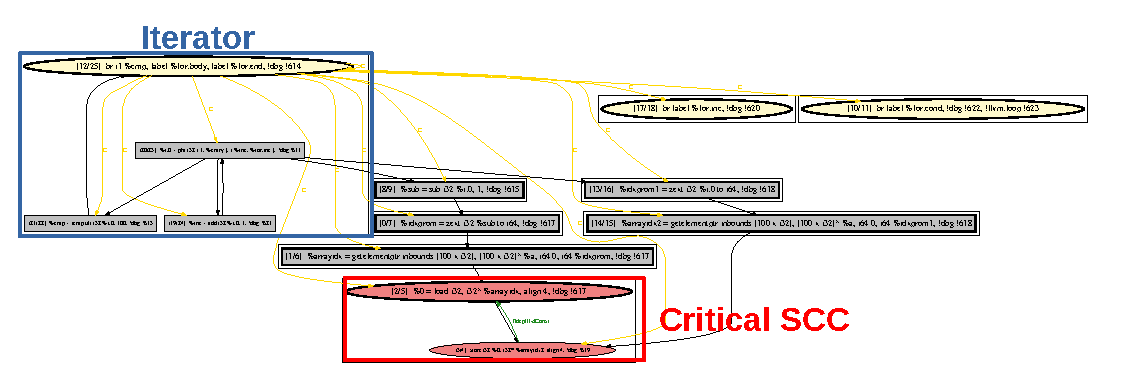
\includegraphics[width=1.0\textwidth]{pdg_example}
\caption{Illustration of a faster convergence to the maximum achievable parallel software performance.}
\label{logo}
\end{figure}

\subsection{Machine Learning Methodology}



\section{Manual Software Parallelisation Assistant}

\begin{figure}
\centering
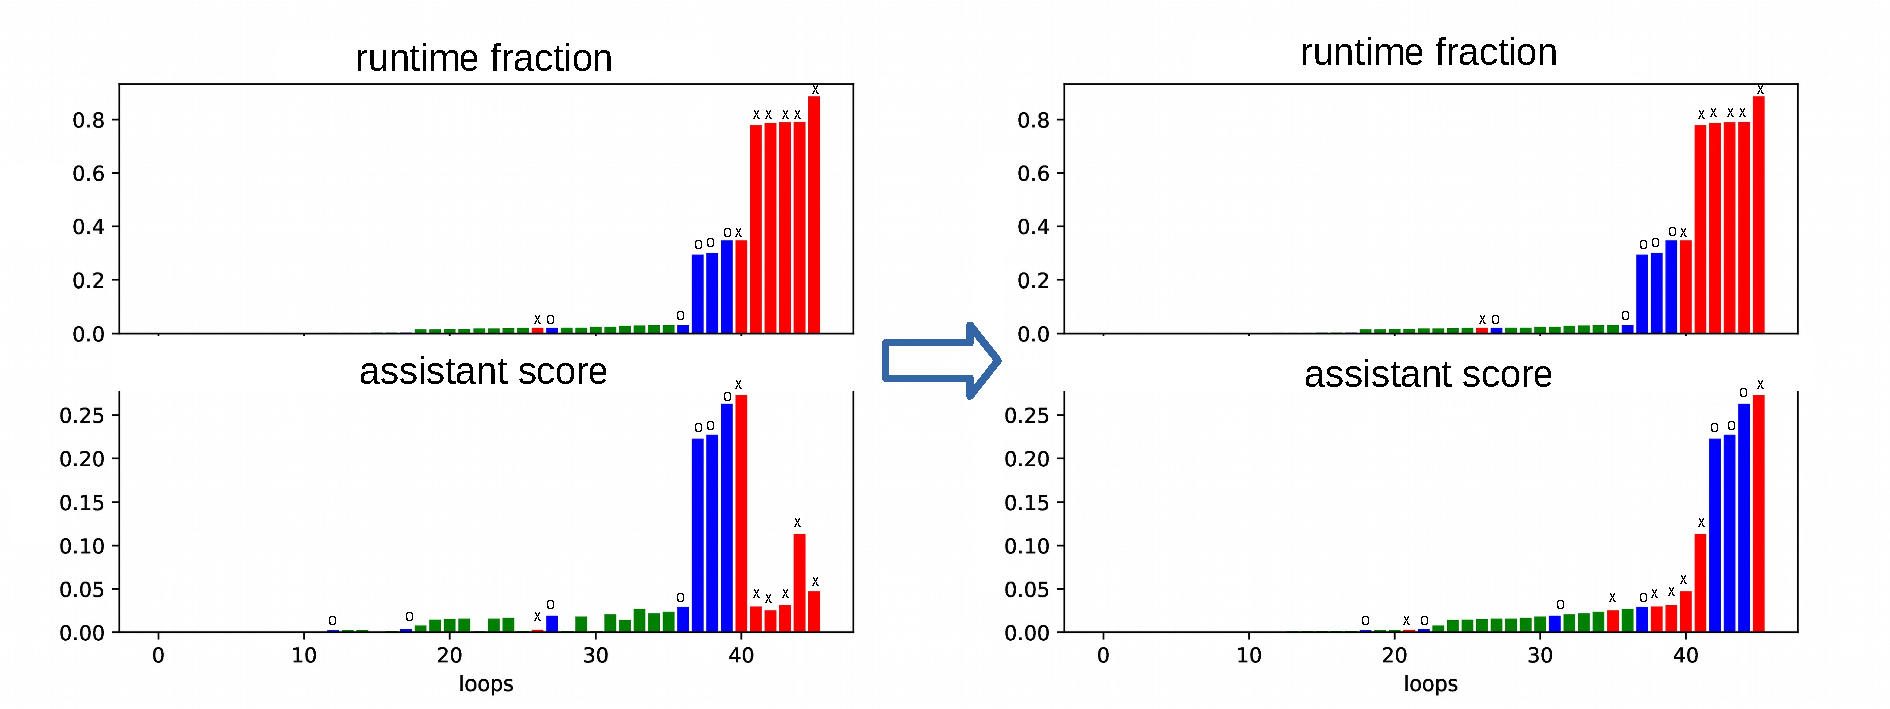
\includegraphics[width=1.0\textwidth]{ft_ranking}
\caption{Illustration of loop ranking transformation.}
\label{logo}
\end{figure}


\section{Evaluation}

\subsection{ML Model Predictive Performance}


\subsection{Assistant Scheme}

\begin{figure}
\centering
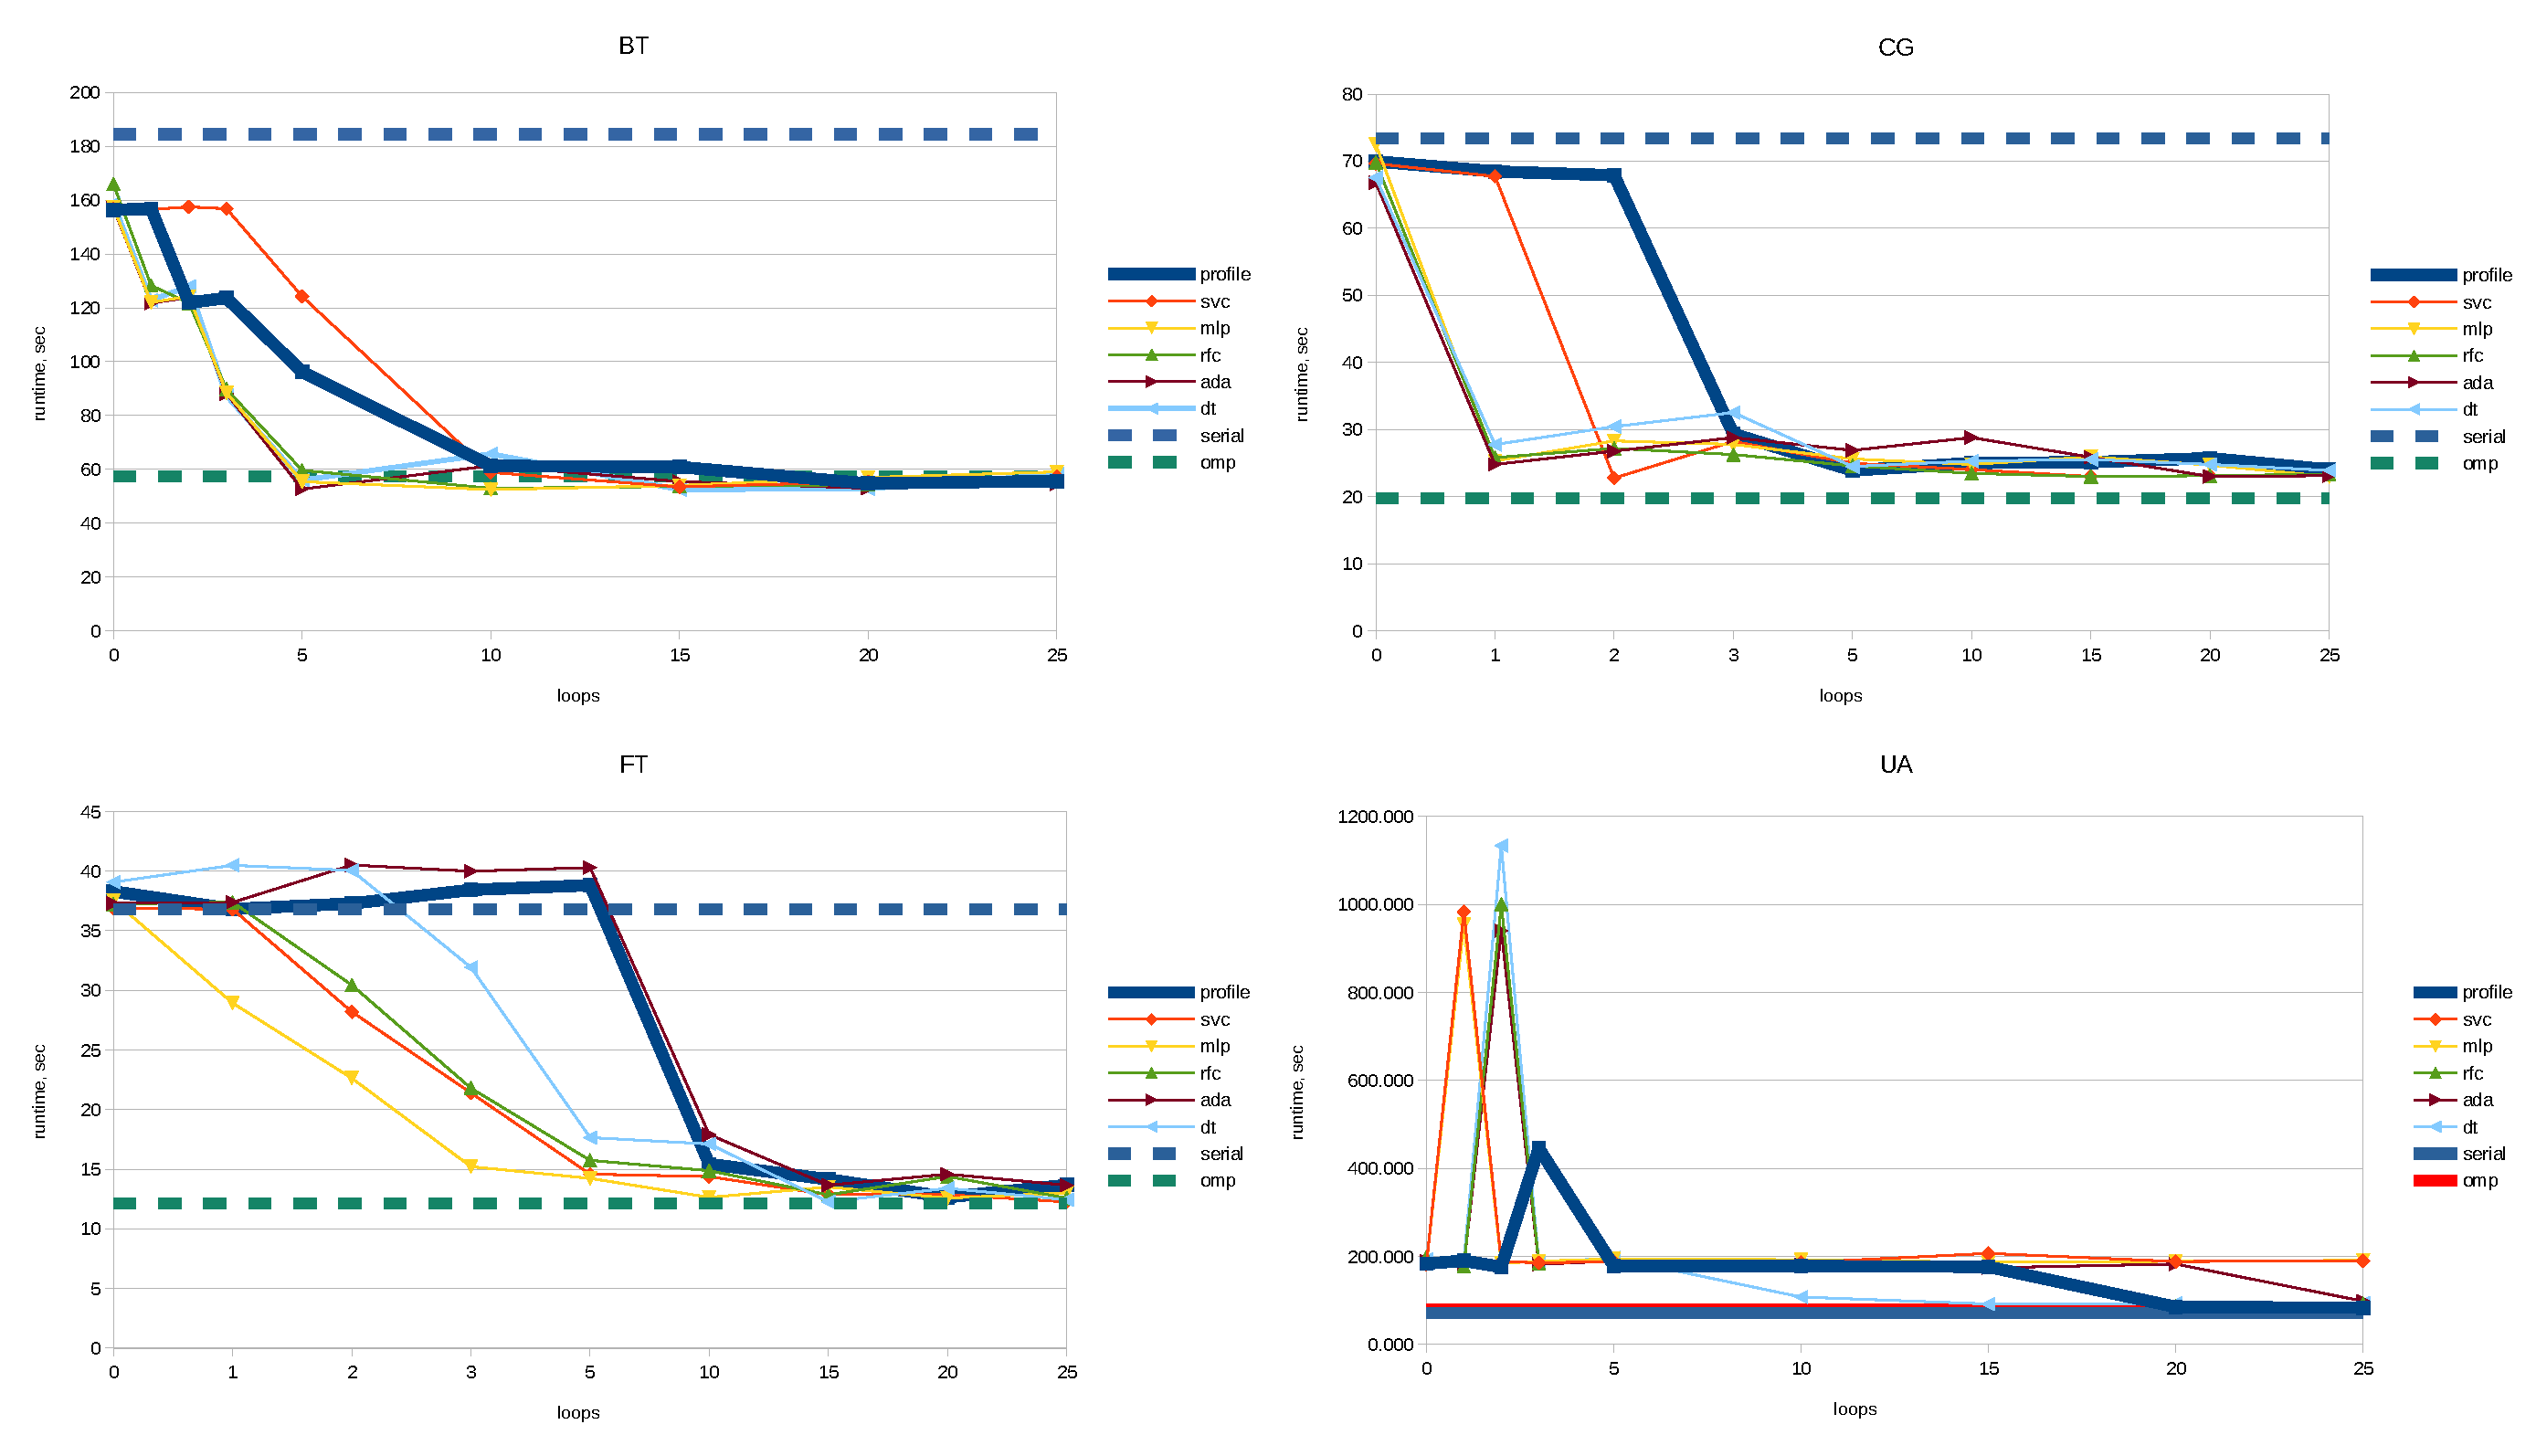
\includegraphics[width=1.0\textwidth]{parallelisation_acceleration}
\caption{Illustration of a faster convergence to the maximum achievable parallel software performance.}
\label{logo}
\end{figure}

\bibliography{guide}

\end{document}

